\documentclass[aspectratio=169,10pt]{beamer}
\usetheme{Madrid}
\usecolortheme{default}
\usepackage[utf8]{inputenc}
\usepackage[T1]{fontenc}
\usepackage[spanish,es-noshorthands]{babel}
\usepackage{booktabs,tabularx,array,graphicx,xcolor,hyperref}
\definecolor{tesisgreen}{HTML}{8BCF45}
\definecolor{tesisdark}{HTML}{111318}
\definecolor{tesisgray}{HTML}{59616B}
\setbeamercolor{structure}{fg=tesisgreen!85!black}
\setbeamercolor{frametitle}{fg=white,bg=tesisdark}
\setbeamercolor{title}{fg=white,bg=tesisdark}
\setbeamercolor{normal text}{fg=tesisdark,bg=white}
\setbeamercolor{block title}{fg=white,bg=tesisdark}
\setbeamercolor{block body}{fg=tesisdark,bg=tesisgreen!9}
\setbeamercolor{alerted text}{fg=tesisgreen!60!black}
\setbeamertemplate{navigation symbols}{}
\setbeamertemplate{itemize item}{\color{tesisgreen}$\bullet$}
\setbeamertemplate{footline}{\hfill\scriptsize\color{tesisgray}UMA–SJL\hspace{0.35cm}\insertframenumber/\inserttotalframenumber\hspace{0.25cm}\vspace{0.2cm}}
\hypersetup{colorlinks=true,urlcolor=tesisgreen!50!black,linkcolor=tesisgreen!50!black}
\title[Enrutamiento predictivo]{Enrutamiento predictivo de estrategias de atención}
\subtitle{Simulación con el banco disponible}
\author{Carlos César Sánchez Coronel \and Freud Enrique Melgar Aliaga}
\institute{Universidad Nacional de Ingeniería · Maestría en Inteligencia Artificial\\Caso de estudio: Facultad de Ingeniería y Negocios, UMA–SJL}
\date{Lima, noviembre de 2026}
\begin{document}

\setbeamercolor{background canvas}{bg=tesisdark}
\begin{frame}[plain]
\vspace{0.7cm}
\vspace{1.1cm}
{\color{white}\LARGE\bfseries ¿Puede la consulta ayudar a elegir\\la estrategia de atención?}\par\vspace{0.45cm}
{\color{white!75}\large Enrutamiento predictivo para consultas\\académico-administrativas}\par\vfill
{\color{white}\normalsize Carlos César Sánchez Coronel · Freud Enrique Melgar Aliaga}\par
{\color{white!65}\small Universidad Nacional de Ingeniería · Lima, 2026}
\end{frame}
\setbeamercolor{background canvas}{bg=white}

\begin{frame}{Problema y pregunta}
\begin{columns}[T]
\begin{column}{.55\textwidth}
\textbf{En los picos del ciclo, la atención manual se vuelve cuello de botella.}
\begin{itemize}
\item Consultas repetidas por ventanilla, correo y mensajería.
\item Unas se responden con documentos; otras requieren reglas, herramientas o criterio humano.
\item Usar siempre la ruta más compleja puede añadir costo sin ayudar a cada consulta.
\end{itemize}
\end{column}
\begin{column}{.40\textwidth}
\begin{block}{Pregunta del estudio}
¿Las señales de la consulta ayudan a seleccionar una estrategia de atención con mejor equilibrio entre calidad, latencia y costo?
\end{block}
\end{column}
\end{columns}
\vfill
\end{frame}

\begin{frame}{2 · Qué medimos en este piloto | 30 s}
\begin{columns}[T]
\begin{column}{.49\textwidth}
\begin{block}{Métrica piloto}
F1 macro para predecir la etiqueta borrador de estrategia. Da el mismo peso a A1, A3 y A5, aunque tengan tamaños distintos.
\end{block}
\begin{itemize}
\item 196 consultas; clases: A1=125, A3=27, A5=44.
\item Etiquetas automáticas/borrador; validación experta pendiente.
\end{itemize}
\end{column}
\begin{column}{.47\textwidth}
\begin{block}{Métricas de tesis aún por medir}
Calidad de respuesta y fidelidad; latencia extremo a extremo; costo por consulta; acierto de derivación y seguridad.
\end{block}
\small Esos resultados no se infieren del F1 del clasificador.
\end{column}
\end{columns}
\end{frame}

\begin{frame}{Protocolo}
\begin{enumerate}
\item Partimos del banco piloto de consultas y de la etiqueta \texttt{candidate\_strategy}.
\item Conservamos la misma tarea y comparamos tres bloques de variables:
\begin{itemize}
\item \textbf{F0:} forma de la pregunta (8 variables).
\item \textbf{F1:} F0 + señales de intención (17 variables).
\item \textbf{F2:} F1 + puntajes BM25 de recuperación (22 variables).
\end{itemize}
\item Para A/B: regresión logística con balanceo de clases; validación estratificada de 5 pliegues; semilla 42.
\item Para HPO: Random Forest sobre F1; 30 pruebas aleatorias + 30 TPE; comparación bajo validación cruzada.
\end{enumerate}
\begin{alertblock}{Lectura del protocolo}
Los pliegues miden predicción de etiquetas piloto. No son todavía corridas de A0–A5 ni mediciones de calidad/costo de respuestas generadas.
\end{alertblock}
\end{frame}

\begin{frame}{Resultado principal: añadir intención ayuda}
\begin{columns}[T]
\begin{column}{.55\textwidth}
\centering
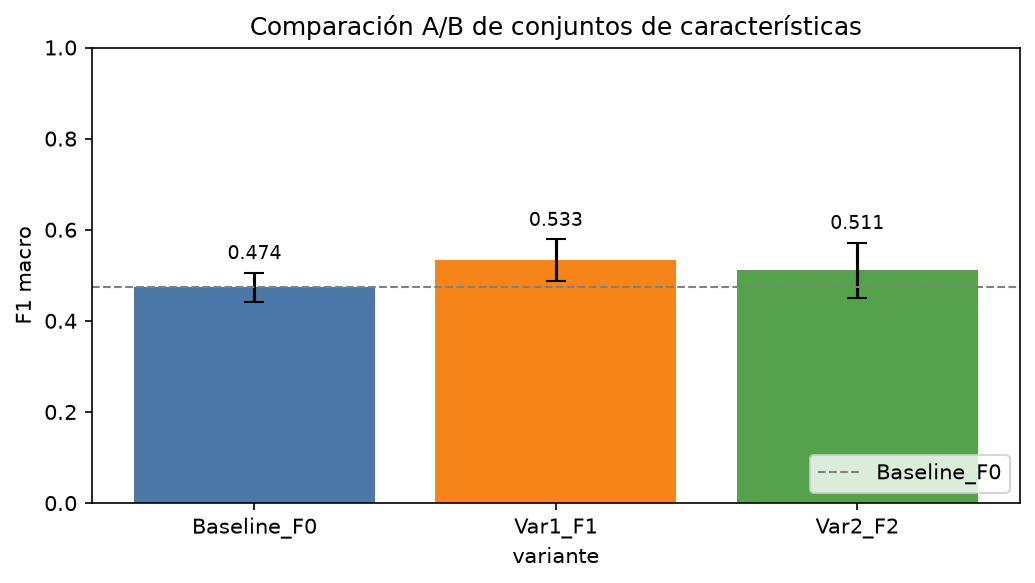
\includegraphics[width=\linewidth]{reports/figures/semana6_ab_f1_barras.png}
\end{column}
\begin{column}{.42\textwidth}
\small
\begin{tabular}{@{}lrr@{}}
\toprule
Variante & F1 macro & Exactitud\\
\midrule
F0 · forma & 0.474 $\pm$ 0.032 & 0.495\\
F1 · intención & \textbf{0.533 $\pm$ 0.046} & \textbf{0.602}\\
F2 · + BM25 & 0.511 $\pm$ 0.061 & 0.577\\
\bottomrule
\end{tabular}
\vspace{0.5em}
\begin{block}{Qué se observa}
F1 supera F0 en 5.9 puntos de F1 macro. Añadir BM25 a F1 no mejora el resultado en este banco.
\end{block}
\end{column}
\end{columns}
\vfill
\scriptsize Media $\pm$ desviación estándar entre cinco pliegues. Misma semilla y modelo; resultados del banco piloto.
\end{frame}

\begin{frame}{Ablación de variables}
\begin{center}
\begin{tabular}{@{}p{2.0cm}p{4.0cm}rrp{4.2cm}@{}}
\toprule
Cambio & Variables añadidas & F1 macro & $\Delta$ vs. F0 & Lectura\\
\midrule
F0 $\rightarrow$ F1 & Señales de intención, entidades y tipo de razonamiento & 0.533 & +0.059 & La intención aporta señal útil para predecir la etiqueta.\\
F1 $\rightarrow$ F2 & Puntajes de recuperación BM25 & 0.511 & $-0.022$ & La señal de recuperación no añadió valor en esta configuración.\\
\bottomrule
\end{tabular}
\end{center}
\vspace{0.45cm}
\begin{block}{Conclusión técnica acotada}
La mejora apunta a enriquecer la descripción de la consulta antes de optimizar el clasificador. No prueba que BM25 sea inútil: faltan revisar cobertura, etiquetas y configuración de recuperación.
\end{block}
\end{frame}

\begin{frame}{Búsqueda de hiperparámetros}
\begin{columns}[T]
\begin{column}{.50\textwidth}
\centering
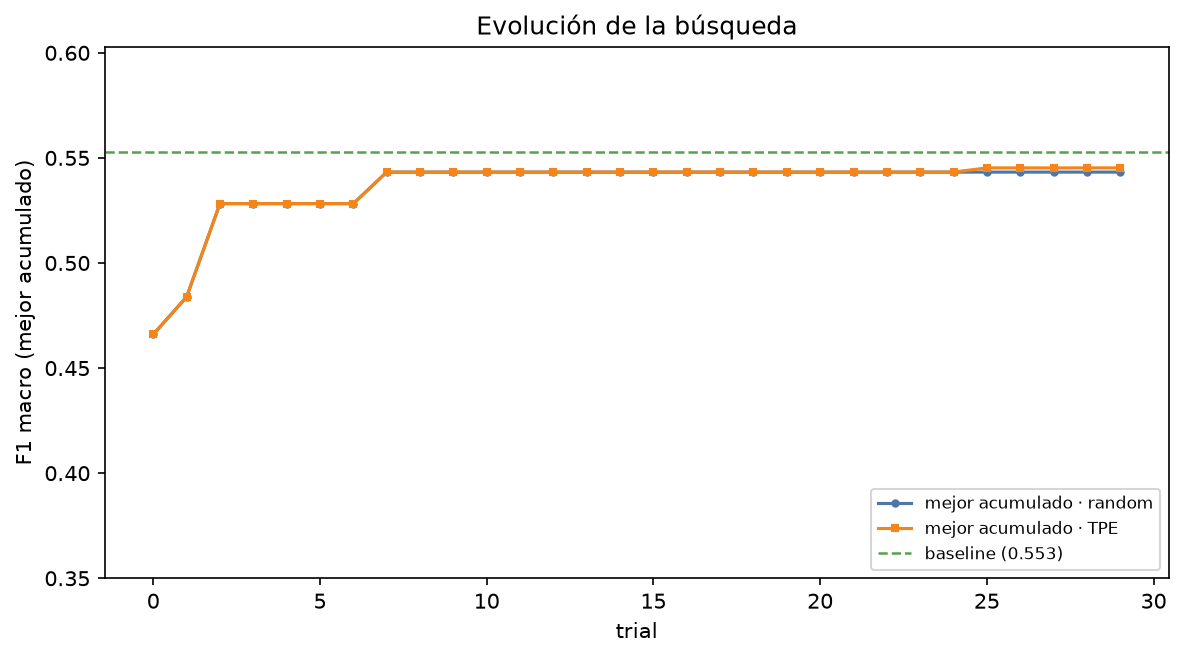
\includegraphics[width=\linewidth]{reports/figures/semana8_hpo_evolucion.png}
\end{column}
\begin{column}{.45\textwidth}
\small
\begin{tabular}{@{}lrr@{}}
\toprule
Random Forest en F1 & F1 macro & DE\\
\midrule
Baseline & \textbf{0.553} & 0.086\\
Mejor aleatorio & 0.543 & 0.048\\
Mejor TPE & 0.545 & 0.059\\
\bottomrule
\end{tabular}
\vspace{0.5em}
\begin{block}{Decisión}
Se conserva el baseline. La búsqueda no mejoró la media; el resultado es sensible al pliegue y al tamaño del banco.
\end{block}
\end{column}
\end{columns}
\end{frame}

\begin{frame}{Riesgos y plan inmediato}
\begin{columns}[T]
\begin{column}{.49\textwidth}
\textbf{Riesgos actuales}
\begin{itemize}
\item Etiquetas en borrador, sin acuerdo de expertos.
\item Desbalance de clases: A1 reúne 64\% de las consultas.
\item Banco piloto pequeño y no representativo.
\item Sin validación de malla vigente ni consultas reales anonimizadas.
\item Sin respuesta generada, A0–A5, latencia ni costo evaluados.
\end{itemize}
\end{column}
\begin{column}{.47\textwidth}
\textbf{Siguiente experimento}
\begin{enumerate}
\item Validar consultas, referencias y rutas con expertos; medir acuerdo.
\item Congelar particiones de calibración y evaluación.
\item Ejecutar A0–A4 en las mismas consultas y registrar calidad, fidelidad, latencia y costo.
\item Comparar R0–R2 y ablacionar intención, recuperación y herramientas.
\item Probar filtro de seguridad y registrar derivaciones correctas.
\end{enumerate}
\end{column}
\end{columns}
\end{frame}

\begin{frame}{Reproducibilidad}
\small
\textbf{Código y artefactos}\par
\href{https://github.com/sanchezclases996/investigaciontesis2}{Repositorio compartido: investigaciontesis2}\par
\vspace{0.25cm}
\textbf{Desde la carpeta \texttt{examen-parcial}:}
\begin{block}{Comandos}
\ttfamily\small
source .venv/bin/activate\\
jupyter nbconvert --execute --to notebook --inplace notebooks/06\_ab\_data\_variants.ipynb\\
jupyter nbconvert --execute --to notebook --inplace notebooks/08\_optimizacion\_hiperparametros.ipynb
\end{block}
\textbf{Semillas y salidas:} semilla 42; cinco pliegues estratificados. Métricas en \texttt{logs/metrics\_experimentos.csv}, \texttt{logs/hpo\_resumen.csv} y decisiones en \texttt{logs/hpo\_decision.csv}.\par
\vspace{0.2cm}
\scriptsize La ejecución de esta presentación corrió las celdas de ambos notebooks. Las corridas completas A0–A5 siguen pendientes.
\end{frame}

\setbeamercolor{background canvas}{bg=tesisdark}
\begin{frame}[plain]
\centering\vfill
{\color{white}\Huge Gracias}
\vfill
\end{frame}
\end{document}
